\chapter{Natural Language Processing}\label{ch_nlp}
\chapterauthor{Ellis Cain}

This chapter introduces natural language processing, with an emphasis on techniques that can be used in conjunction with neural networks. A dominant theme throughout the chapter is the concept of a word embedding (section \extref{wrangling}), where words in a corpus are associated with vectors that capture important characteristics. This makes it possible to associated words and texts with activations that can be processed in a neural network. These techniques have a long history in linguistics and in the study of neural networks, but have become especially prominent in recent years with the advent of large language models like GPT (section \extref{transformers}). We will also see that pre-processing (section \extref{wrangling}) is important with linguistic data, shedding further light on the general topic of wrangling data before it is used in a neural networks.

% Formally a word embedding  is a function from a set of tokens to a set of vectors in an n-d space. 

\section{Background and History}

\subsection{Linguistics}

Linguistics is the study of language, which can be organized by the different aspects of language, going from smallest to largest unit of study: \textbf{phonetics} and \textbf{phonology} as the study of speech sounds, \textbf{morphology} as the study of words and form, \textbf{syntax} as the study of the structure or grammar (usually at the sentence level), \textbf{semantics} as the study of meaning, which can be at a variety of levels (words, phrases, sentences), \textbf{pragmatics} as the study of intentional meaning or implied meaning (think Gricean maxims and rules of conversations). 
% TODO: Convert the above into glossary items, or unboldface

The smaller units of study are generally straightforward for analysis, looking at phonemes (smallest unit of sound, /t/ or /p/) or morphemes (smallest word unit of meaning, ``luck'' in ``unlucky''), as you increase the scope of analysis it increasingly becomes more difficult to (automatically) analyze. For syntax, there are treebanks and dependency analyzers that have to be trained on lots of example hand-annotated data to be able to analyze new sentences. There are also reasonable limits per word (for syntactic analysis), a word usually has one or two parts of speech (noun, verb, determiner, etc.), and there are constructed rules for how to derive dependency trees. What about meaning for semantics? There isn't a clear unit of ``meaning'' for words, a meaning is more broad, it can be abstract or concrete (``justice'' vs ``cup''), it can be flexible and change based on the context (``bass'' as the fish or instrument). How could we automate the analysis of semantic information?

% Something about computational linguistics and tools? WordNet is a lexical database of English constructed by linguists, where words are organized into ``synsets'' (cognitive synonyms or groups of words). Similarity is calculated using the Wu-Palmer path similarity function which is based on the number of jumps between synsets.


\subsection{Early word embeddings}

% TODO: Check and fix
One early approach was to simply manually create feature vectors based on linguistic attributes.  For example, in Elman's ``Finding structure in time''~\cite{elman1990finding}, each of 6 words was associated with a 31-bit vector.  Some examples are shown in figure \ref{elmanWordEmbeddings}.

\begin{figure}[h]
\centering
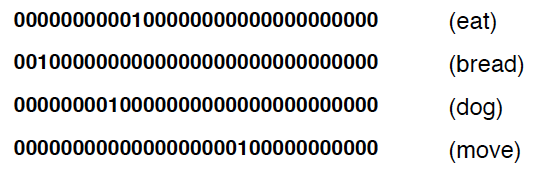
\includegraphics[scale=.5]{./images/elmanWordEmbeddings.png}
\caption[From \cite{elman1990finding}.]{Some of Elman's word embeddings. }
\label{elmanWordEmbeddings}
\end{figure}

These early embeddings were hand-crafted based on the scientist's intuitions or using other simple techniques to ensure certain similarity structures. However, automated forms of word embedding are also available. These automated approaches take documents and use the information in them to produce word embeddings.

% There is a historical trajectory from document level down to word level. 

One simple idea in the background of many word embeddings is the \glossary{Bag of words} approach, which associates documents with vectors of word frequencies. This approach ignores grammatical structure and just looks at how often different tokens occur in different documents. We take our document, put each token in the document in a bag, and count up how many tokens occur in each bag.  Consider the following documents

\begin{description}
\item[Document 1]  ``The bass fish played the bass''
\item[Document 2]  ``The fish played fish with the fish monger''
\end{description}

Bag of words will associate these as follows

\begin{table}[h]
    \centering
    \begin{tabular}{|l|c|c|c|c|c|c|}
    \hline
    Document & the & bass & fish & played & with & monger \\
    \hline
    Document 1 & 2 & 2 & 1 & 1 & 0 & 0 \\
    Document 2 & 3 & 0 & 3 & 1 & 1 & 1 \\
    \hline
    \end{tabular}
    \caption{Bag of words representation}
\end{table}

A slightly more complex document level embedding is TF-IDF (term frequency-inverse document frequency), which is used to calculate the importance of a specific term for a (set of) related document(s), which offsets how frequently a term appears (term frequency) by the number of other documents that also contain the term. This allows it to focus on meaningful terms and not those that generally appear frequently. 


% Dictionary representation. (``The bass fish played the bass'' would be {``the'': 2, ``bass'': 2, ``fish'': 1, ``played'': 1}).

This document term frequency approach. We pass a sliding window over the terms of a document and do the same procedure as bag of words but where the ``document'' is a term and the vector is the frequency count in the window around that term, which can be thought of as a co-occurrence vector.  In the example above suppose window size is 1.  Then we scan across the two documents and see that ``the'' co-occurs twice with ``bass'',  twice with ``fish'', once with ``played'', and once with ``with''.  The full set of word embeddings is:

% TODO
%\begin{table}[h]
%    \centering
%    \begin{tabular}{|l|c|c|c|c|c|c|}
%    \hline
%    Term & the & bass & fish & played & with & monger \\
%    \hline
%    the 1 & 2 & 2 & 1 & 1 & 0 & 0 \\
%    Document 2 & 3 & 0 & 3 & 1 & 1 & 1 \\
%    \hline
%    \end{tabular}
%    \caption{Word Occurrence Frequencies}
%\end{table}

To begin to get a feel for some of this ideas see \url{http://vectors.nlpl.eu/explore/embeddings/en/}
 
\section{Distributional Semantics Theory}

% Methods mentioned above deal more with a surface-level analysis of language from text; term analysis, etc.

% TODO Make bibtex entries
The theory of distributional semantics (Firth, 1957; Harris, 1954) and other usage-based theories of language (Wittgenstein, 1953) posit that the usage of words reflects their meaning, and information about the meaning of words is embedded in linguistic context and the statistical properties of language usage.

This is often illustrated with the following quote, due to John First: ``You shall know a word by the company it keeps.'' For example, when someone talks about a \textit{river}, they may also mention \textit{water} or \textit{bank} (as in river bank), helping the listener correctly decode the intended meaning.

By connecting usage to meaning, this allows for an approximation or representation of meaning that is derived from usage in a text corpora. Instead of analyzing large corpora by hand, computational algorithms can be used to generate numeric representations.

\subsection{Document-level semantic analysis}

LSA (latent semantic analysis): used with a body (set) of documents to analyze semantic information and calculate document similarity. The body of documents are represented using a document term matrix, where each row corresponds to a document, and each column is the frequency of a given term in each document. Then, singular value decomposition (SVD) is used for dimensionality reduction, resulting in a numeric vector for each document (based on term usage/frequency) which can be compared using cosine similarity (section \extref{dotProduct}) to get document similarity.

\subsection{Word-level semantic analysis}

Algorithms like Word2Vec (Mikolov et al., 2013) are used to track the linguistic context and word co-occurrences to ``embed'' words into a semantic space, much like our own semantic space (Lewis et al., 2019), where the words can be tracked and compared. 

\begin{figure}[h]
    \centering
    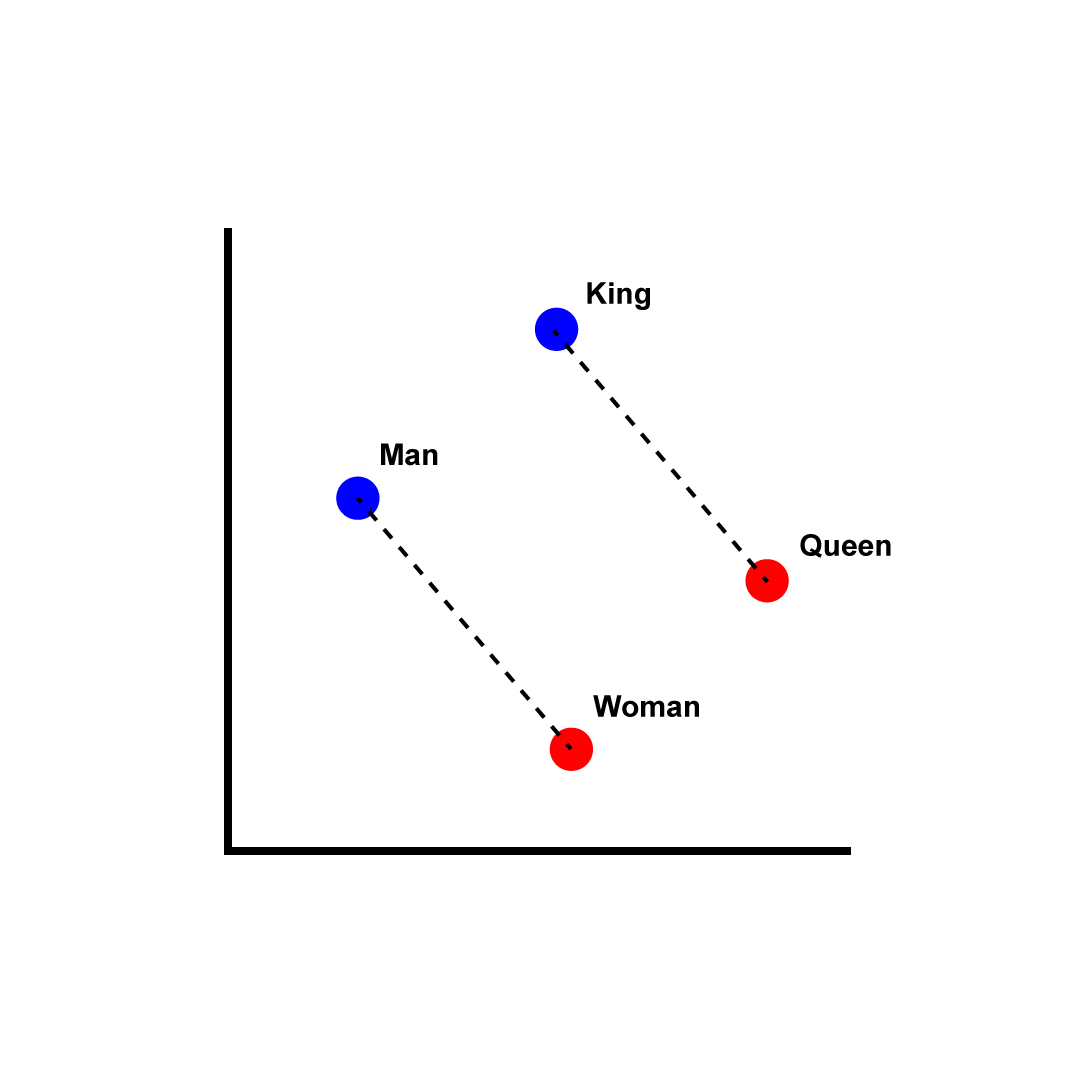
\includegraphics[scale=.2]{./images/Word_vector_illustration.jpg}
    \caption[From \url{https://en.wikipedia.org/wiki/Word2vec\#/media/File:Word_vector_illustration.jpg}.]{Example of word embeddings in a semantic space. A hypothetical embedding for the four words ``king'', ``queen'', ``man'', and ``woman''.  The embedding makes sense because we would expect that the representation of ``king'' to be closer to ``man'' than to ``woman'', ``queen'' should be closer to ``woman'' than to ``man'', and the distance between ``man'' and ``king'' should be the same as that between ``queen'' and ``woman''.    }
 \label{f:kingQueenExample}
\end{figure}

% \textit{Brunila \& LaViolette's paper revisiting the idea of distributional semantics: \url{https://arxiv.org/pdf/2205.07750.pdf} (URL for now \dots)}

\section{Word Embeddings and Co-occurrence Matrices}

As noted in the discussion of data wrangling (section \extref{wrangling}), data must often be preprocessed before it can be used in a neural network. In the case of linguistic data this is an extremely important topic involving multiple steps.  

Take this sentence, for example: ``Footsteps shuffled on the stair. Under the firelight, under the brush, her hair spread out in fiery points glowed into words, then would be savagely still.'' (From T. S. Eliot's \textit{The Waste Land})

Data preparation and processing in NLP generally follows this pipeline: 

\begin{enumerate}
\item Sentence segmentation
\item Word tokenization
\item Normalization and filtering
\item Main analysis
\end{enumerate}

For sentence segmentation, the paragraph or document is segmented into sentences. This step is particularly important when using text that has been scanned using OCR, where errors might occur.

Once the document has been segmented into sentences, a tokenizer is used to split each sentence into the comprising words. 

Following tokenization, the words/tokens are generally normalized to remove capitalization or certain punctuation marks, such that the words are consistently in the same form.

In this step, ``stopwords'' (words that are deemed insignificant; usually function words) can also be filtered out.

Depending on your research goal, the exact implementation of this pipeline will differ.

% After segmentation and tokenization: 
% [[footsteps,shuffled,on,the,stair], 
% [under,the,firelight,under,the,brush,her,hair,
% spread,out,in,fiery,points,glowed,into,words,
% then,would,be,savagely,still]] \textit{Formatting?}

After segmentation and tokenization: 
\begin{quote}
[[footsteps, shuffled, on, the, stair], 
[under, the, firelight, \dots, savagely, still]]
\end{quote}

Once the text has been preprocessed, the main analysis can proceed. For a very basic word embedding algorithm, the label-context pair co-occurrences are tracked in a co-occurrence matrix.

Each word is iterated as the `label', while the surrounding words serve as the `context'. A window size is defined, which designates how many words to include in the `context'. Skip-gram models will include context both before and after a given label.

From our example, we may start out with ``footsteps'' as the label, then if we have a window size of two, the co-occurring label-context pairs would be [footsteps, shuffled] and [footsteps, on].
Then, when we get to ``on'' as the label, the label-context pairs would include [on, footsteps], [on, shuffled], [on, the], [on, stair].

Once the document has been processed, the result is a co-occurrence matrix where each cell represents the raw co-occurrence counts for a given label-context pair.

\subsection{Example}

Not every word is used with the same frequency, so some determiners (`the', `a') may be over-represented and skew the co-occurrence matrix. If these type of stopwords were not removed, we can change the weight of different contexts. Therefore, a positive-pointwise mutual information transform is often used to weight the matrix. 

\textbf{From simbrain documentation:} Weights the co-occurrence values to avoid word-frequency-bias in embeddings. Words like ``the'' and ``a'' that should not be considered meaningful in terms of co-occurrence are down-weighted. Less frequent words on the other, like ``platitude'' or ``espresso'', that are more meaningful in terms of co-occurrences, are up-weighted.

\textbf{Quote from Lenci:} PPMI measures how much the probability of a target-context pair estimated in the training corpus is higher than the probability we should expect if the target and the context occurred independently of one another. (Lenci, 2018)

\textit{See Lenci review paper for in-depth explanation and discussion.}

The result is a set of \textit{n}-dimensional vectors for a set of words, which are referred to as ``word embeddings.''

\subsection{Evaluation}

How then should these embeddings be evaluated? 

Previous research on word similarity and relatedness has shown that directly asking for relatedness judgements can accurately capture word relations (Finkelstein et al. 2002).

Therefore, the general method of evaluation is by collecting a set of human judgements, which theoretically serve as the ceiling of model of model performance. \textit{Check paper that reviewer mentioned? https://aclanthology.org/2022.bionlp-1.26/}

There are a variety of gold standards that have been used across the field, such as WordSim-353 or MEN (citations), however, recent models have already reached or surpassed human performance on these tasks.

Therefore, Hill and colleagues set out to create a gold standard that separates similarity from association, which previous standards had ignored the distinction.

For example, ``car'' and ``tire'' would be considered associated but not similar, ``glasses'' and ``spectacles'' would be considered similar. See Hill et al., 2014 for an in-depth discussion.

\subsection{Corpus quality}

While different algorithms may improve the model performance and similarity to our own semantic representations, the corpus quality also has an impact on model performance.
Larger training corpora generally improve the quality of the derived embeddings. 
GloVe embeddings are trained on various trainint corpora, varying from 1 billion tokens to 42 billion tokens (from the Common Crawl) \textit{Citations.}

Beside the amount or size of the training corpora, the type of documents is also important; training solely on works of fiction would lead to different embeddings than a model trained on non-fiction, and so on. It is important to consider the meaning you are trying to capture (generalized or specific to a field, such as medical documents).

\section{Relation to neual networks}
Above mentioned methods mainly track co-occurrence frequencies, which reflect statistical learning theories (SL citations), where learners track label-object co-occurrence statistics.
There is also another line of theory in linguistics called predictive processing, where individuals predict future input. This has been used to combat Chomsky's argument about negative evidence (citation), since through disconfirmed predictions, individuals can ``create'' their own negative evidence to learn from (citation for further discussion?).

% Alternative training method using neural networks
In a similar fashion, neural networks have also been used to generate word embeddings.


% Data processing using neural networks


% Large language models, reference other chapter

\section{Exercises}

\subsection{Basic NLP}

\begin{enumerate}
\item Walkthrough a simple example of counting co-occurrences.
\item How does window size impact the embeddings?
\item What is potential motivation for using the \textit{skip-gram} setting?
\item Calculate the similarity between these words: [list of words]. 
\item Something about the PPMI transformation?
\end{enumerate}

\subsection{Geometric thinking}

\begin{enumerate}
\item What does it mean for a word embedding to be n-dimensional?
\item Why is cosine similarity used over other distance functions, like traditional euclidean distance?
\item Something where they perform clustering?
\end{enumerate}

\subsection{Corpus quality}

\begin{enumerate}
\item With the limited (demo) training corpus, how well do you think it captures the actual meaning of the words?
\item Does corpus size or quality matter? (Too basic of a question.)
\item Something with a corpus that deals with polysemy (financial institution \& geographic texts)
\end{enumerate}

\subsection{Neural Networks and other advances}

\begin{enumerate}
\item SRNs?
\item Next-word prediction?
\item Text generation?
\end{enumerate}